\newpage

\section{Propuesta}

Establecidos estos puntos, implementaremos los algoritmos en un sistema de alto nivel. Aunque los siete algoritmos analizados tienen la misma finalidad, difieren en su estructura, lo que afecta el tiempo y la cantidad de operaciones necesarias. Aplicaremos estos siete algoritmos en los siguientes tres lenguajes de programación: Python, Java y C++. También se presentará una comparación gráfica usando datos que van desde 100 hasta 100,000 elementos en una lista.

\subsection{Bubble Sort} 
Cpp
\lstinputlisting[language=C++]{code/bubble.cpp}

Java
\lstinputlisting[language=Java]{code/bubble.java}

\vspace{5cm}
Python
\lstinputlisting[language=Python]{code/Bubble.py}

\begin{figure}[h]
    \centering
    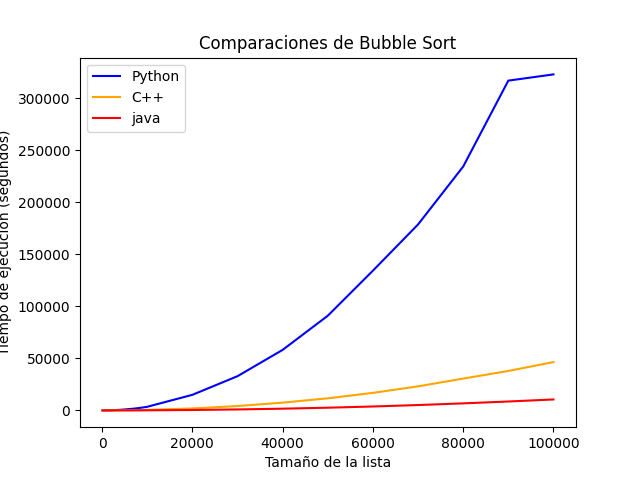
\includegraphics[scale=.60]{img/bubble sort.png}
    \caption{Comparaciones de Bubble Sort en C++,Java y Python}
    \label{fig:primera_figura}
\end{figure}

\subsection{Selection Sort}
Cpp
\lstinputlisting[language=C++]{code/selection.cpp}
Java
\lstinputlisting[language=Java]{code/selection.java}
\vspace{1cm}
Python
\lstinputlisting[language=Java]{code/selection.py}

\begin{figure}[h]
    \centering
    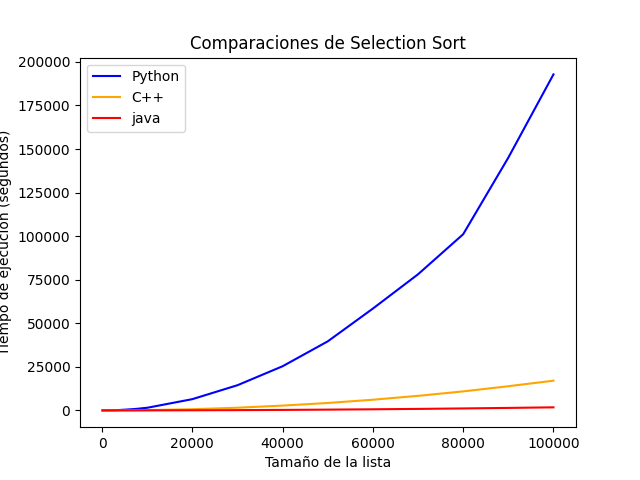
\includegraphics[scale=.60]{img/Selection Sort.png}
    \caption{Comparaciones de Selection Sort en C++,Java y Python}
    \label{fig:primera_figura}
\end{figure}

\subsection{Insertion Sort} 
Cpp
\lstinputlisting[language=C++]{code/insertion.cpp}
Java
\lstinputlisting[language=Java]{code/insertion.java}

\vspace{4cm}
Python
\lstinputlisting[language=Python]{code/insertion.py}

\begin{figure}[h]
    \centering
    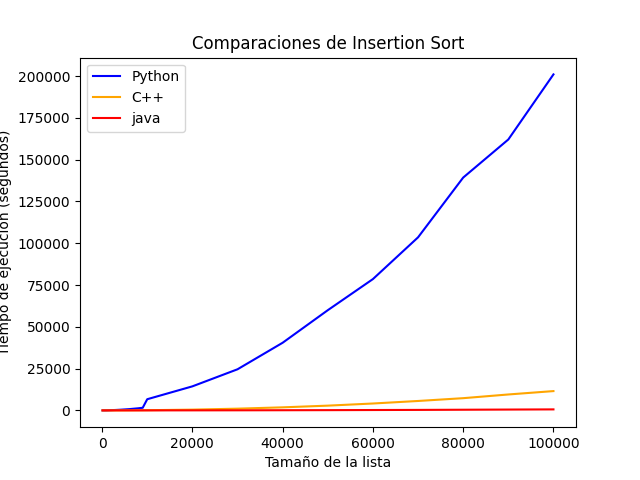
\includegraphics[scale=.60]{img/Insertion sort.png}
    \caption{Comparaciones de Insertion Sort en C++,Java y Python}
    \label{fig:primera_figura}
\end{figure}

\subsection{Counting Sort} 
Cpp
\lstinputlisting[language=C++]{code/counting.cpp}
Java
\lstinputlisting[language=Java]{code/counting.java}
Python
\lstinputlisting[language=Python]{code/counting.py}

\begin{figure}[h]
    \centering
    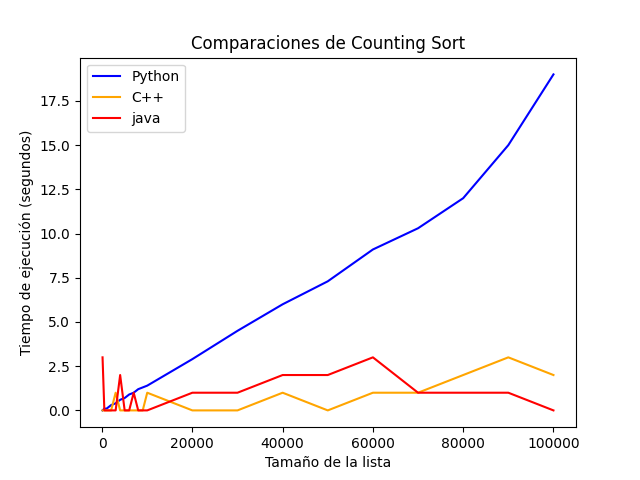
\includegraphics[scale=.60]{img/counting sort.png}
    \caption{Comparaciones de Counting Sort en C++,Java y Python}
    \label{fig:primera_figura}
\end{figure}

\subsection{Heap Sort} 
Cpp
\lstinputlisting[language=C++]{code/heap.cpp}
\vspace{3cm}
Java
\lstinputlisting[language=Java]{code/heap.java}

Python
\lstinputlisting[language=Python]{code/heap.py}

\begin{figure}[h]
    \centering
    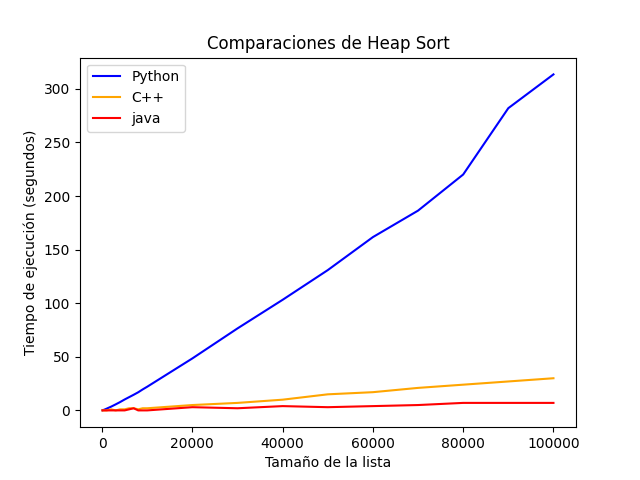
\includegraphics[scale=.60]{img/heap sort.png}
    \caption{Comparaciones de Heap Sort en C++,Java y Python}
    \label{fig:primera_figura}
\end{figure}

\subsection{Merge Sort} 
Cpp
\lstinputlisting[language=C++]{code/merge.cpp}
Java
\lstinputlisting[language=Java]{code/merge.java}
Python
\lstinputlisting[language=Python]{code/merge.py}

\begin{figure}[h]
    \centering
    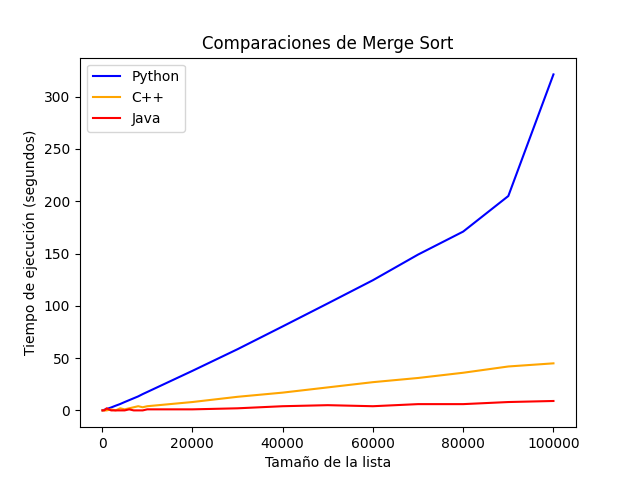
\includegraphics[scale=.60]{img/merge sort.png}
    \caption{Comparaciones de Merge Sort en C++,Java y Python}
    \label{fig:primera_figura}
\end{figure}

\vspace{2cm}
\subsection{Quick Sort} 
Cpp
\lstinputlisting[language=C++]{code/quick.cpp}
Java
\lstinputlisting[language=Java]{code/quick.java}
Python
\lstinputlisting[language=Python]{code/quick.py}

\begin{figure}[h]
    \centering
    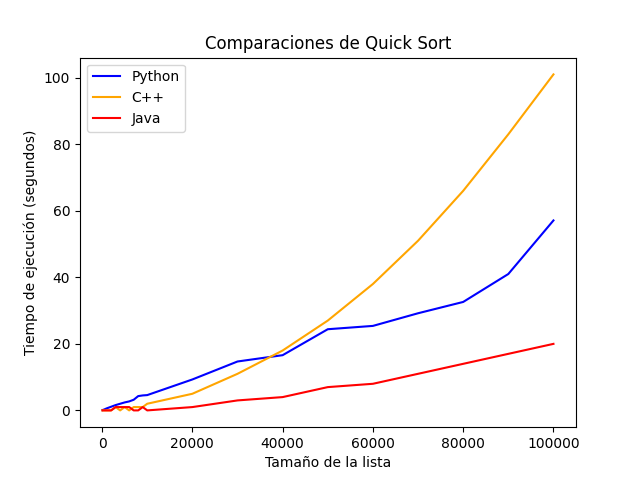
\includegraphics[scale=.60]{img/quick sort.png}
    \caption{Comparaciones de Quick Sort en C++,Java y Python}
    \label{fig:primera_figura}
\end{figure}

Una vez graficados cada algoritmo en cada lenguaje, a continuación se mostrarán los siete algoritmos de ordenación implementados previamente en los tres lenguajes: C++, Java y Python.

\begin{figure}[h]
    \centering
    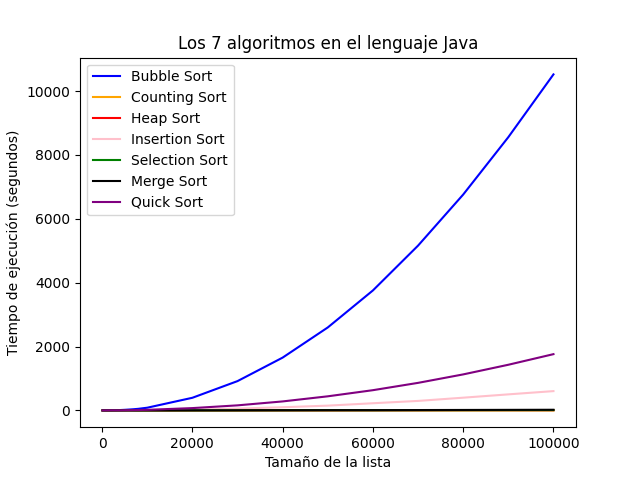
\includegraphics[scale=.60]{img/Java.png}
    \caption{Los 7 algoritmos en Java}
    \label{fig:primera_figura}
\end{figure}

\vspace{2cm}
\begin{figure}[h]
    \centering
    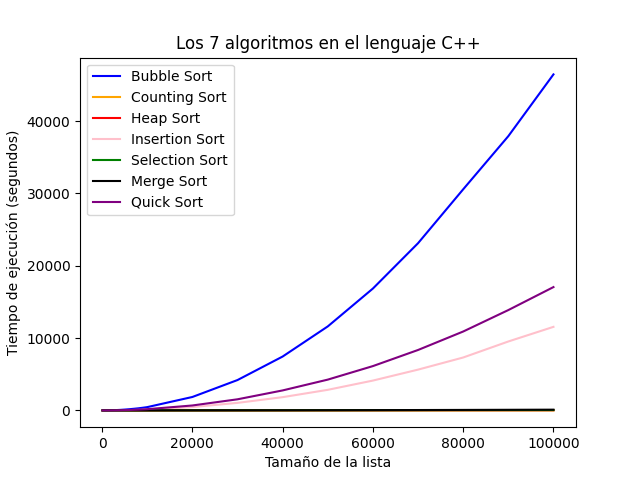
\includegraphics[scale=.60]{img/CPP.png}
    \caption{Los 7 algoritmos en C++}
    \label{fig:primera_figura}
\end{figure}

\begin{figure}[h]
    \centering
    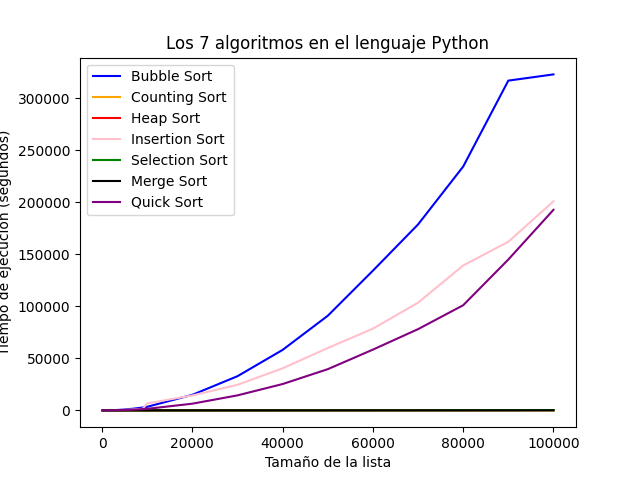
\includegraphics[scale=.60]{img/Python.png}
    \caption{Los 7 algoritmos en Python}
    \label{fig:primera_figura}
\end{figure}
